\section{并发模型}
\begin{frame}{分叉--汇合(Fork-Join)模型}
  \begin{columns}
      \column{.5\textwidth}
        \begin{itemize}
          \item 程序执行过程中,\alert{父线程}可以分叉出与其并发执行的\alert{子线程}
          \item \alert{汇聚点}: 子线程从独立执行到汇合回父线程的时间点
        \end{itemize}

      \column{.5\textwidth}
      \begin{figure}
        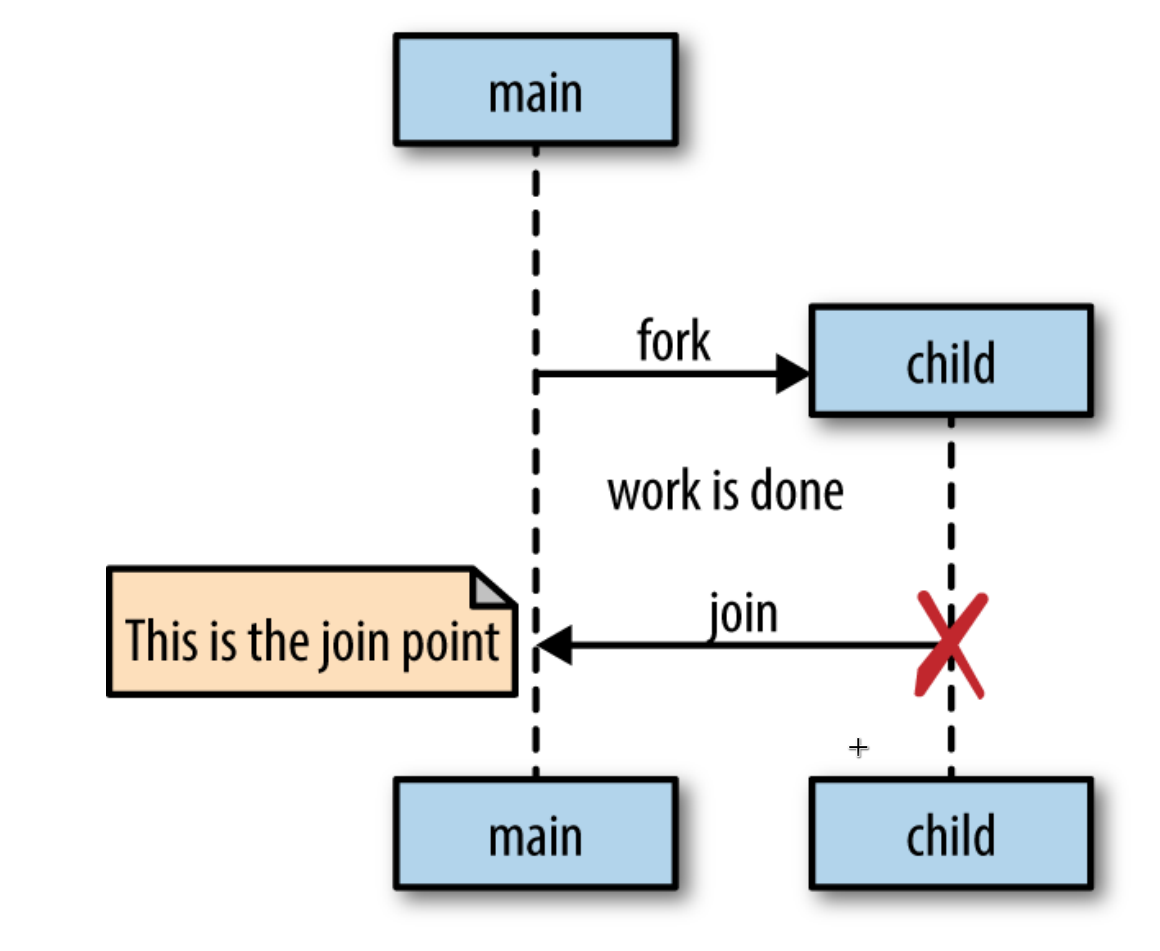
\includegraphics[width=\textwidth]{images/fork-join.png}
        \caption{分叉--汇合模型}
      \end{figure}
  \end{columns}
\end{frame}

\begin{frame}[fragile]{错误设置的汇聚点}
\begin{lstlisting}[caption={不正确的汇聚点引发竞态},label={wrong-join}]
sayHello := func() {
  fmt.Println("hello")
}
go sayHello()
// continue doing other things
\end{lstlisting}

    \alert{以上程序的输出结果是不确定的}。因为协程由 Go 的运行时创建和调度,\texttt{sayHello}协程没能通过合适的汇聚点和主协程进行汇合,因此,如果被调度之前主协程已退出,\texttt{sayHello}就无法获得执行的机会

    \begin{exampleblock}{温馨提示}
        \textbf{正确设置的汇聚点}能确保程序正确性并消除潜在的\alert{竞态} 
    \end{exampleblock}
\end{frame}

\begin{frame}[fragile]{纠正的汇聚点}
为上述程序设置正确的汇合点,\texttt{sayHello}必须和主协程\textbf{同步},使自己能在主协程退出之前与其汇合,解决方案之一如\lstlistingname~\ref{lst-ok-join}

\begin{lstlisting}[caption={利用同步确保\texttt{sayHello}在主协程退出之前与其汇合},label=lst-ok-join]
var wg sync. WaitGroup
sayHello := func() {
  defer wg.Done()
  fmt.Println("hello")
}
wg.Add(1)
go sayHello()
wg.Wait()  // 汇聚点

// 输出:
// hello    
\end{lstlisting}

\alert{可见,分叉--汇合模型下并发编程的正确性依赖于数据同步}
\end{frame}

\begin{frame}{数据同步方式}
\texttt{go}语言实现数据同步操作提供了两种方式
\begin{itemize}
    \item 传统地,\alert{共享内存型同步模式},常用元件分布在\texttt{sync}包
    \item \alert{基于顺序进程通信(CSP)}的消息传递实现数据同步,主要元件为通道\texttt{channel}及\texttt{select}语句
\end{itemize}
\end{frame}